\documentclass{anstrans}

%%%% packages and definitions (optional)
\usepackage{graphicx} % allows inclusion of graphics
\usepackage{booktabs} % nice rules (thick lines) for tables
\usepackage{microtype} % improves typography for PDF
\usepackage{float}
\usepackage{subcaption}
\usepackage{booktabs}
\usepackage{tikz}
\usepackage{afterpage}
\usetikzlibrary{shapes.geometric, arrows,shapes.arrows,calc,positioning}

\newcommand{\SN}{S$_N$}
\renewcommand{\vec}[1]{\bm{#1}} % vector is bold italic
\newcommand{\vd}{\bm{\cdot}} % slightly bold vector dot
\newcommand{\grad}{\vec{\nabla}} % gradient
\newcommand{\ud}{\mathop{}\!\mathrm{d}} % upright derivative symbol


%%%% changes from the original 'anstrans' class
\usepackage{fancyhdr} % allows headers and footers

\renewcommand\headrule{} % remove underline in the header
\setcounter{secnumdepth}{1}
\renewcommand{\thesection}{\Roman{section}.}
\renewcommand{\thesubsection}{\arabic{subsection}.}
\renewcommand{\thesubsubsection}{\Alph{subsubsection}.}
\makeatletter
\renewcommand*{\@seccntformat}[1]{\csname the#1\endcsname\hspace{1mm}}
\makeatother


%%%% Header
\pagestyle{fancy}
\fancyhf{}
\fancyhead[L]{\fontsize{9}{9} \itshape
M\&C 2017 - International Conference on Mathematics \& Computational Methods Applied to Nuclear Science \& Engineering,
\\ Jeju, Korea, April 16-20, 2017, on USB (2017)
}


%%%% Maketitle
\title{Residual Monte Carlo Transport in Time with Consistent Low-Order Acceleration for
    1D Thermal Radiative Transfer}
\author{Simon R.~Bolding,$^{*}$ Jim E.~Morel$^{\dagger}$} 
\institute{
$^{*}$Los Alamos National Laboratory, Los Alamos, NM \\
$^{\dagger}$Texas A\&M University Nuclear Engineering Department, College Station, TX}

\email{sbolding@tamu.edu \and morel@tamu.edu}

% My documents
\newcommand{\N}{\mathbb{N}}
\newcommand{\Z}{\mathbb{Z}}
\newcommand{\deriv}[2]{\frac{\mathrm{d} #1}{\mathrm{d} #2}}
\newcommand{\pderiv}[2]{\frac{\partial #1}{\partial #2}}
\newcommand{\bx}{\mathbf{X}}
\newcommand{\ba}{\mathbf{A}}
\newcommand{\by}{\mathbf{Y}}
\newcommand{\bj}{\mathbf{J}}
\newcommand{\bs}{\mathbf{s}}
\newcommand{\B}[1]{\ensuremath{\mathbf{#1}}}
\newcommand{\Dt}{\Delta t}
\renewcommand{\d}{\mathrm{d}}
\newcommand{\mom}[1]{\langle #1 \rangle}
\newcommand{\xl}{{x_{i-1/2}}}
\newcommand{\xr}{{x_{i+1/2}}}
\newcommand{\il}{{i-1/2}}
\newcommand{\ir}{{i+1/2}}
\newcommand{\keff}{\ensuremath{k_{\text{eff}}}}
\newcommand{\sig}[1]{\ensuremath{\Sigma_{#1}}}
\newcommand{\ra}{\ensuremath{\rightarrow}}
\newcommand{\dd}{\ensuremath{\mathrm{d}}}
\renewcommand{\O}{\ensuremath{\mathbf{\Omega}}}
\newcommand{\adj}{\ensuremath{{}^{\dagger}}}
\newcommand{\x}{\ensuremath{\mathbf{x}}}
\newcommand{\T}{\ensuremath{\text{T}}}
\newcommand{\iso}[2]{$^{#2}$#1}
\newcommand{\phibar}{\ensuremath{\overline{\phi}}}
\newcommand{\cur}[1]{\left\{ #1 \right\}}
\newcommand{\jl}{{j-1/2}}
\newcommand{\jr}{{j+1/2}}
\newcommand{\E}[1]{\ensuremath{\operatorname{E}_{#1}}}
\newcommand{\rface}{\ensuremath{r_{\text{face}}}}
\newcommand{\FOM}{\ensuremath{\text{FOM}}}
\newcommand{\ds}[0]{\displaystyle}
\newcommand{\invcm}[0]{cm$^{-1}$}
\renewcommand{\u}[1]{\ensuremath{\underline{#1}}}
\newcommand{\dep}{\ensuremath{\delta\epsilon^{(m)}}}
\renewcommand{\ss}{\ensuremath{\|s\|}}
\newcommand{\pos}{{\text{pos}}}
\newcommand{\phsp}{\ensuremath{\left(\mathbf{r},\mathbf{\Omega},\nu,t\right)}}
\newcommand{\Del}{\ensuremath{\nabla}}


%%%% Abstract
\begin{document}
\vspace*{-42pt}
\begin{strip}
\centering{\parbox{153mm}{{\bf Abstract} \itshape - 
We have extended a high-order low-order (HOLO) algorithm for thermal radiative transfer problems to include Monte Carlo (MC) integration of
the time variable. Within each discrete time step, fixed-point iterations are performed between a
high-order (HO) exponentially-convergent Monte Carlo (ECMC) solver and a low-order (LO)
system of equations.  The ECMC algorithm integrates 
the angular intensity over a time step, and the low-order (LO) radiation equations are closed consistently
in the time variable. The time closure increases accuracy in optically-thin problems compared to
a backward Euler discretization.  The LO system is based on spatial
and angular moments of the transport equation and a linear-discontinuous
finite-element (LDFE) spatial representation, producing equations similar to the standard
S$_2$ equations.   The emission source is fully implicit in time, and Newton iterations efficiently resolve the nonlinear
temperature dependence of the LO equations at each time step.  
 The HO solver computes angular and temporal consistency terms that preserve the accuracy
 of the MC integration in the LO equations.  We have implemented the ECMC algorithm with linear
 and constant, doubly-discontinuous trial spaces.   Numerical results demonstrate that the second discontinuity in the
 time variable is necessary for sufficient consistency to achieve stable convergence, for the chosen closure of the LO
 equations.
 Results are compared to an implicit Monte Carlo (IMC) code and the HOLO algorithm with a BE time
 discretization.  One-dimensional, gray test problems were tested
for a range of optical thicknesses.  The HOLO algorithm is more efficient and accurate than IMC with sufficient mesh
resolution and number of particle histories.
}\par}
\vspace*{14pt}
\end{strip}

%%%%%%%%%%%%%%%%%%%%%%%%%%%%%%%%%%%%%%%%%%%%%%%%%%%%%%%%%%%%%%%%%%%%%%%%%%%%%%%%
\section{Introduction}

Accurate solutions to the thermal radiative transfer (TRT) equations are important for simulations
in the high-energy, high-density physics regime, e.g., for inertial confinement fusion and
astrophysics.  Computational modeling of TRT problems features coupling between
a photon radiation field and a high-temperature material, where energy is exchanged through
absorption and emission of photons by the material.  Typical applications often require solution in
a mix of streaming and diffusive regions due to absorption-emission physics and
cross sections that are a function of material temperature.  In this work, we improve on the
time-integration accuracy of a high-order low-order (HOLO) method in optically thin regions where
particles stream without undergoing many interactions, while preserving the computational efficiency
of a residual MC HO solver in optically thick regions.

Moment-based hybrid Monte Carlo (MC)
methods have demonstrated great potential for accelerated
solutions to TRT problems~\cite{rmc,bolding_nse,holo_rh}.   These nonlinear acceleration methods iterate between a
high-order (HO) transport equation and a low-order (LO) system formulated with angular moments
and a fixed spatial discretization.  Physics operators that
are expensive for the HO solver to resolve directly in tightly coupled problems, e.g., photon absorption and emission,
are moved to the LO system. The lower-rank LO equations can be solved with Newton
methods to allow for nonlinearities in the LO equations to be efficiently
resolved~\cite{willert,bolding_nse}.  The high-order (HO) problem is defined by the radiation transport equation with
isotropic sources computed with the previous LO solution. A MC transport solution to the HO
problem is used to construct consistency terms that appear in the LO equations. These consistency terms preserve the accuracy of the HO
solution in the next LO solve, as the two solutions iteratively converge.

Previously, residual MC methods have been used to provide efficient
solution to the HO transport problem~\cite{rmc,bolding_nse}; high-fidelity solutions,
with minimal statistical noise, have been achieved for problems with optically-thick, diffusive
regions that lead to slowly varying
solutions.  However, the algorithms in previous work have used a backward
Euler (BE) discretization for the time variable.  The BE discretization can inaccurately disperse radiation
wavefronts in optically thin problems, leading to inaccuracies. 

We have extended the algorithm in~\cite{bolding_nse} to include higher-accuracy MC treatment of the time variable for the
radiation unknowns.  The exponentially-convergent Monte Carlo (ECMC)
algorithm was modified to include integration of the time variable;
this includes the introduction of a step, doubly-discontinuous (SDD) trial space representation in
time.  We have also investigated a linear,
doubly-discontinuous (LDD) and a linear-discontinuous
(LD) projection in time.  The overall higher-dimensionality of the linear spaces requires development of a 
modified sampling approach that should be useful for extending the ECMC algorithm to higher spatial
dimensions.  A new
parametric closure of the LO equations, introducing additional time-closure consistency
terms, was derived to capture the time accuracy of the HO
ECMC simulations.  The LO equations can preserve the accuracy of the ECMC radiation transport treatment in
time, with the same numerical expense as Backward Euler (BE) time-discretized S$_2$
equations. We have derived the LO equations directly from the transport equation
such that, neglecting spatial discretization differences,
the HO and LO solutions are consistent upon convergence, preserving space-angle-time moments.
Herein we briefly describe the algorithm, and we present results for
one-dimensional (1D), grey test problems.  We compare our method to the implicit MC
(IMC) method~\cite{fnc} for accuracy and statistical efficiency for several representative problems.
%%%%%%%%%%%%%%%%%%%%%%%%%%%%%%%%%%%%%%%%%%%%%%%%%%%%%%%%%%%%%%%%%%%%%%%%%%%%%%%%

\subsection{Thermal Radiative Transfer Background and IMC}

The continuous 1D, grey TRT equations consist of the radiation and
material energy rate equations, i.e.,\vspace{-0.05in}
\begin{align}\label{ho_cont}
 \hspace{-0.12in}   \frac{1}{c}\pderiv{I(x,\mu,t)}{t} + \mu \pderiv{I(x,\mu,t)}{x} &+ \sigma_a
    I(x,\mu,t)
= \frac{1}{2} \sigma_a a c T^4(x,t)
    \\ \label{t_cont}
  \rho c_v \pderiv{T(x,t)}{t} &=  \sigma_a \phi(x,t) - \sigma_a a c T^4(x,t),
\end{align}
with appropriate initial and boundary conditions specified.
%with specified isotropic initial and boundary conditions for $t>0$:
%\begin{align}
%    I(x,\mu,0) &= I^0(x), & 0\leq x \leq X \\ 
%    I(0,\mu,t) &= I^+_{inc}, & 0 \leq \mu \leq 1 \\ 
%    I(0,\mu,t) &= I^+_{inc}, & 0 \leq \mu \leq 1 \\ 
%\end{align}
In the above equations, $x$ is the position, $t$ is the time, $\mu$ is
the $x$-direction cosine of the angular intensity $I(x,\mu,t)$, $\sigma_a$ is the
macroscopic absorption cross section (cm$^{-1}$), and $a$, $c$, $\rho$,
and
$c_v$ are the radiation constant, speed of light, mass density, and specific heat,
respectively.  Physical scattering could be included in Eq.~\eqref{ho_cont}, but it is omitted
for brevity and simplicity.  The desired transient unknowns are the material
temperature $T(x,t)$ and the scalar radiation intensity $\phi(x,t)=\int_{-1}^1
I(x,\mu,t)\, \d \mu$.  The scalar intensity is related to the radiation energy density
$E_r$ by the relation $E_r = \phi/c$.  The equations can be 
strongly coupled through the gray Planckian emission source $\sigma_a a c T^4$, which
is a nonlinear function of temperature, and the absorption
term $\sigma_a \phi$.  In optically thin problems, with small $\sigma_a$, the solution becomes
increasingly linear as the emission source becomes negligible.

We will compare results in this work to the implicit Monte Carlo (IMC) method.  The IMC
method~\cite{fnc} is the standard approach for solution of the TRT equations with Monte Carlo particle
transport~\cite{wollaber_review}.  The IMC method partially linearizes the system of equations over
a discrete time step, with material properties evaluated at the previous-time-step temperature. The
linearized system produces a transport equation with an approximate emission source and an effective scattering cross section representing
absorption and re-emission of photons over a time step~\cite{fnc}. This transport equation is advanced over a
time step via a MC simulation.   The MC transport simulation tallies energy absorption over a discretized spatial mesh,
which can be used to directly estimate a spatially discretized representation of the end of time step material temperature.
%In optically thick regions, or for large time steps, the effective scattering
%dominates interactions.  In these diffusive regions IMC becomes computationally expensive.

For this work, we are primarily interested in comparing to the time discretization of IMC.
The material temperature and emission source are discretized with an implicit time discretization,
i.e., a BE discretization.  However, because the linearization is approximate, the system is not
truly implicit, and there is a limit on the time step size to produce physically accurate
results in problems that are tightly coupled and strongly nonlinear~\cite{wollaber2013discrete}. 
The linearized equations are integrated over the $n$-th time step defined for
$t\in[t^{n-1/2},t^{n+1/2}]$, with width $\Delta t=t^{n+1/2}-t^{n-1/2}$ and center $t^{n}=t^{n-1/2} +
\Delta t/2$. The radiation equation is solved via MC simulation of particle histories, with the time-averaged
energy deposition tallied over the spatial mesh.    The time-integrated radiation equation, in nonlinear form, is
\begin{multline}
I^{n+1/2}(x,\mu) - I^{n-1/2}(x,\mu) = \\ \Delta t \left[\sigma_a^{n-1/2} \overline{I}(x,\mu) - {\mu
\pderiv{\overline{I}(x,\mu)}{x}} 
+\frac{1}{2} \sigma_a a c \left(T^{n+1/2}\right)^{4}(x) \right].
\end{multline}
The end-of-time-step intensity $I^{n+1/2}(x,\mu)\equiv I(x,\mu,t^{n+1/2})$ is stored as ``census''
particles that have reached $t^{n+1/2}$,
representing a continuous sample of the phase space at that particular time~\cite{fnc}, to be used in the next
time step.  In strongly diffusive regions, the accuracy will be limited to first
order by the time discretization of the temperature terms.  However, in optically-thin regions, higher-accuracy for the 
radiation terms is achieved.
It is noted that the time-averaged effective scattering source resulting from
linearization of the emission source in IMC is treated approximately in the time variable to allow
the MC simulation to simulate the isotropic scattering events~\cite{wollaber_review,fnc}.

\subsection{The High-Order Low-Order Algorithm}

Previously, we have developed a HOLO algorithm for 1D TRT problems, based on BE time-discretized
HO and LO equations~\cite{bolding_nse}.
In the time-discrete HOLO algorithm, the LO solver resolves the time-discrete material
temperature spatial distribution $T^{n+1/2}(x)$ over each time step, whereas the HO solver computes weighted
angular integrals of the intensity.  The HOLO formulation has several desirable
properties.  In particular,  the LO solver can efficiently converge nonlinearities in diffusive
systems, without the need to solve the nonlinear equations with MC simulation.
Because the nonlinearities are converged, the temperature and emission source
have a truly implicit discretization, preserving the discrete maximum principle~\cite{morel_mpv}.
Additionally, by using the ECMC HO solver, solutions with minimal statistical noise can be achieved
efficiently, preventing instability issues that may be introduced through noise in the consistency terms.

To achieve temporal accuracy similar to IMC, we compute weighted temporal integrals of the
intensity with the HO solver, used for computing additional consistency terms.
We must assume a time discretization for the temperature field to produce a linear HO transport problem
with closable LO equations.  As in the IMC method, a BE time discretization is applied to
emission source throughout, but the radiation variables are left in terms of time-averaged and
end-of-time-step unknowns.   Currently, our residual
formulation requires a space-angle LDFE projection of the solution in order to estimate
$I(x,\mu,t^{n+1})$, rather than the continuous sample represented by the census in IMC.
This projection can be inaccurate with insufficient mesh resolution in near-void problems.
However, the LDFE projection of the solution, estimated with MC inversion of the linear transport operator,
will greatly increase the accuracy over a standard finite-difference
discretization of the radiation equation.  The HOLO algorithm should still demonstrate improvement over IMC in efficiency and
accuracy in problems with intermediate and large optical thickness. 

The fully-discrete LO equations are based on space-time-angle moments of the TRT equations, formed
over a spatial finite-element (FE) mesh.  Angularly, the LO radiation equations are similar to S$_2$
equations,  with element-averaged consistency parameters that are time-averaged, intensity-weighted averages of $\mu$.  The
angular treatment is analogous to the hybrid method in~\cite{wolters}. A lumped LDFE spatial discretization (e.g., see~\cite{morel_ldtrt}) is used to close the system
spatially. Additional consistency parameters must be introduced to the LO equations to eliminate the
auxiliary time-unknowns from the LO radiation equations.  The additional time consistency terms are
based on parametric modifications to a standard time discretization.  Once closed, a system of
equations is formed for the primary moment unknowns. If the angular and time consistency parameters
were exact, then the LO equations would produce the exact moments of the solution, neglecting
spatial discretization differences between the two systems.  The HO consistency parameters are
lagged in each LO solve. The LO equations always conserve energy, independent of the accuracy of the consistency terms.

The solution to the LO system is used to construct a spatially LDFE, and temporally constant,
representation of the emission source on the right hand side of Eq.~\eqref{ho_cont}.  This defines a
fixed-source, pure absorber transport problem for the HO operator.  This HO transport problem is
solved with the ECMC algorithm. The HO transport problem can be viewed as a characteristic
method, where we are using ECMC to invert the continuous-streaming, time-derivative, and removal
operators~\cite{bolding_nse}. The ECMC
algorithm is an iterative residual MC method that uses
batches of MC histories to estimate the error in the current trial-space estimate of 
$I(x,\mu,t)$.  It is noted that because we are not using
mesh adaptation in this work, exponential convergence in iterations cannot generally be maintained,
but reduced variance overall can still be achieved. The initial guess for each solve is based on the
solution from the previous time step, which allows for efficient reduction of statistical noise in
problems with minimal change over the time step. The output from ECMC is a projection $\tilde I(x,\mu,t)$ of the intensity onto
the chosen finite-element trial space, i.e., the functional representation of the intensity. Once
computed, $\tilde{I}(x,\mu)$ is used to directly evaluate the necessary LO angular and time-closure
consistency parameters.   The HO solution is not used to directly estimate a new temperature at the
end of the time step, which eliminates the need to linearize the emission source for stability.

Iterations between the HO and LO solves can increase accuracy in strongly nonlinear
problems. However, for the problems tested here, only a single HO solve is performed during each
time step.  Thus, the HOLO algorithm, for the $n$-th time step, is
\begin{enumerate}
    \item Perform a LO solve to produce an initial guess for $T_{LO}^{n+1/2}(x)$
        and $\phi_{LO}^{n+1/2}(x)$, based on angular consistency terms estimated with
        $\tilde{I}^{n-1/2}(x,\mu)$ and a BE time discretization.
\item Solve the HO system for $\tilde{I}_{HO}(x,\mu,t)$ using ECMC, based on the current
    LO estimate of the emission source.%$\sigma_s(T^k)\phi^{k}$ and $B(T)^{k}$.
\item Compute LO angular and time-closure consistency parameters with
    $\tilde{I}_{HO}(x,\mu,t)$.  
\item Solve the LO system using HO consistency parameters to produce a new
    estimate of $\phi^{n+1/2}_{LO}$ and $T^{n+1/2}_{LO}$.
\item Store $\tilde{I}^{n+1/2}(x,\mu)\rightarrow\tilde{I}^{n-1/2}(x,\mu)$, and move to the next time step.
\end{enumerate}

\section{The LO System}
\label{sec:lo}

We will define the LO equations and closure before detailing the HO solver that is used to compute
consistency terms present in the LO equations.
To derive the LO equations, we reduce the dimensionality of Eq.~\eqref{ho_cont} and
Eq.~\eqref{t_cont} by taking spatial, angular, and
temporal integrals.  We will then introduce approximations to
close the system, while being as consistent with the HO solver as possible. 

The spatial domain is divided into $N_c$ uniform spatial cells.
The spatial moments are taken over each spatial cell $i$:
$x\in[x_{i-1/2},x_{i+1/2}]$, weighted with the standard linear FE basis functions.  For example, the left moment operator is defined by
\begin{equation}\label{x_mom}
    \mom{\cdot}_{L,i} = \frac{2}{h_i} \int_{x_{i-1/2}}^{\xr} b_{L,i}(x) (\cdot) \d x,
\end{equation}
where $h_i=x_{i+1/2}-x_{i-1/2}$ is the width of the spatial element and
$b_{L,i}(x)=(x_{i+1/2}-x)/h_i$ is the basis function corresponding to position
$x_{i-1/2}$.  The right moment is defined with basis function $b_{R,i}(x)=(x - x_{i-1/2})/h_i$.
Angularly, the equations are integrated over the positive and negative half
ranges.  The angular integrals of the intensity are defined as $\phi^\pm(x) = \pm2\pi
\int_0^{\pm 1} I(x,\mu) \d \mu$.  Finally, the equations are integrated over the $n$-th
time step defined for $t\in[t^{n-1/2},t^{n+1/2}]$ with width $\Delta t = t^{n+1/2}-t^{n-1/2}$ and
center $t^{n}$.  

The $L$ and $R$ moments and $+$ and $-$ half-range integrals are applied in pair-wise combination to
Eq.~\eqref{ho_cont}, followed by integration over the time step.  After algebraic manipulation, this
ultimately produces 4 moment equations per spatial element.  The streaming terms 
in the resulting equations are manipulated to form averages of $\mu$, weighted with basis functions
and the time-averaged intensity, analogous to previous work~\cite{bolding_nse,wolters}. 
The emission source and temperature-dependent cross sections are approximated with a BE discretization to help close the system.
For example, application of the $\mom{\cdot}_{L,i}$ moment with the positive half-range integral to
Eq.~\eqref{ho_cont} ultimately yields
\begin{multline}\label{eq:t_moml_ex}
    \frac{\mom{\phi}_{L,i}^{+,n+1/2} - \mom{\phi}_{L,i}^{+,n-1/2}}{c \Delta t}
    -2\overline {\mu}_{i-1/2}^{\,+} \overline \phi_{i-1/2}^{\,+} + \overline{\cur {\mu}}_{L,i}^{+}
  \mom{\phibar}_{L,i}^{+}
  +  \overline{\cur\mu}_{R,i}^{+}
  \mom{\phibar}_{R,i}^{+} \\+  \sigma_{a,i}^{n+1/2} h_i 
  \mom{\overline\phi}_{L,i}^{n+1/2,+}  = \frac{h_i}{2} \mom{\sigma_a^{n+1/2} a c T^{n+1/2,4}}_{L,i},
\end{multline}
where over-barred quantities represent the exact averaging over the time step.
A more thorough derivation and definitions for all of the  moment equations can be found in~\cite{dissertation}.

At this point, the only approximation has been the BE time-discretization of the emission source in
both governing equations. 
The face- and volume-averaged angular consistency terms, e.g., $\overline{\mu}_{i-1.2}^+$, were
formed only through algebraic manipulation.   They are approximated with angular intensity from the
previous HO solve.
For example, the $L$ and $+$ time-averaged consistency term is
\begin{equation}\label{eq:cons}
    \overline{\cur{{\mu}}}_{L,i,HO}^{+} \simeq  \frac{\ds 
        {\displaystyle \frac{2}{h_i\Delta t}} \int\limits_{t^{n-1/2}}^{t^{n+1/2}} \int\limits_0^1 \int\limits_\xl^\xr \mu \, b_{L,i}(x)
\tilde I_{HO}(x,\mu,t) \dd x \dd \mu \dd t } 
{\ds {\displaystyle \frac{2}{h_i \Delta t}}\int\limits_{t^{n-1/2}}^{t^{n+1/2}} \int\limits_0^1 \int\limits_\xl^\xr \, b_{L,i}(x)
\tilde I_{HO}(x,\mu,t) \dd x \dd \mu \dd t },
\end{equation}
where $\tilde I_{HO}(x,\mu,t)$ is a space-angle-time finite element projection of the HO intensity,
to be later defined. It is noted that this consistency term contains no division by $\sigma_a$, so
these equations are directly valid in a void.

For simplicity, the face terms $\phi_{i\pm1/2}^\pm$ are eliminated from the
system using a lumped LDFE spatial approximation, with standard upwinding~\cite{bolding_nse}.  The
emission source is also represented with a lumped LDFE interpolant. 
There is some inconsistency introduced in the lumped LDFE spatial approximations. Assuming
iterative convergence of consistency terms, the LO solution and projection of the HO solution may
differ for any given spatial mesh, but the two solutions will converge as the mesh is refined.  This
approximation has proven stable for problems tested and demonstrates preservation of the equilibrium diffusion
limit~\cite{dissertation}. Boundary conditions are incorporated through upwinding and the face term
resulting from integration of the streaming operator.

The material energy equations are similarly integrated in space and time.  
The lumped LDFE approximation is introduce for $T(x)$ and $T^4(x)$ to close the equation spatially, along
with the BE time discretization for the emission source.  The $L$ moment temperature equation is 
\begin{multline}\label{eq:Tt_moml_ex}
     \frac{\rho_i c_{v,i}}{\Delta t}\left[T_{L,i}^{n+1/2} - T_{L,i}^{n-1/2}\right]   + \sigma_{a,i}^{n+1/2} \left( \mom{\phibar}_{L,i}^+ +
    \mom{\phibar}_{L,i}^- \right) \\ = \sigma_{a,i}^{n+1/2}a c
\left( T_{L,i}^{n+1/2}\right)^4,
\end{multline}
where cross sections have been evaluated at $t^{n+1/2}$ and $T_{L,i}$ and $T_{R,i}$ are the LD edge
values of the temperature, e.g., $T(x)=b_{L,i}(x)T_{L,i}+b_{R,i}(x)T_{R,i}$ for
$x\in(\xl,\xr)$.  

\subsection{Parametric Time Closure with HO information}

At this point, there is still too many unknowns in the LO equations. 
Quantities at $t^{n-1/2}$ are known from the previous time step or an initial condition, but a
a relation is needed between the time-averaged radiation quantities and their corresponding values at $t^{n+1/2}$.
The closure of each LO equation  must account for inconsistencies in the
time-discretization of the two solvers. 
Previous work, applied to radiation-hydrodynamics problems, has enforced
consistency in time by adding a local artificial source to the time-discretized LO
equations in each cell~\cite{holo_rh}.  This
source was based HO estimate of the difference in the integral treatments of the time
derivative between the HO and LO systems.  The advantage
of this form is that the LO solver exclusively deals in
time-averaged unknowns for the radiation terms in the equations. 
%However, it may not be sufficiently
%consistent for problems where the difference between the two time integrations is large..
Alternatively, we will use a local, parametric closure to directly eliminate the auxiliary temporal
radiation unknowns, introducing additional consistency terms.

Equation~\eqref{eq:t_moml_ex} will only contain time-averaged radiation unknowns 
if $\mom{\phi}_{L,i}^{n+1/2}$ is eliminated from the
system.  The simplest closure is a weighted average
\begin{equation}\label{eq:time_param}
    \mom{\phi}_{L,i}^{+,n+1/2} \approx \gamma_{L,i,HO}^+ \mom{\overline{\phi}}_{L,i}^+,
\end{equation}
where $\gamma_{L,i,HO}^+$ is a time-closure consistency parameter.  The consistency
parameter can be determined from Eq.~\eqref{eq:time_param} by using moments of $\overline{I}_{HO}(x,\mu)$ and
$I^{n+1/2}_{HO}(x,\mu)$, i.e.,
\begin{equation}
    \gamma_{L,i,HO}^+ = \frac{\mom{\phi_{HO}}_{L,i}^{+,n+1/2}}{\overline{\phi}_{L,i,HO}^+}.
\end{equation}
Because the time-closures account for the different spatial moment equations, there is four per
spatial cell.  For a linear problem, as long as the HO solution used to compute this closure satisfies the same moment
equations as the LO system, or is at least \emph{an accurate approximation to the moment equations},
then the closure relation will stably provide consistency.

The unknowns of interest are $\mom{\overline{\phi}}_{L,i}^\pm$,
$\mom{\overline{\phi}}_{R,i}^+$, $T_{L,i}^{n+1/2}$, and $T_{R,i}^{n+1/2}$. 
The four spatially-closed radiation moment equations per cell, the HO approximation of the
angular consistency terms, the two temperature moment equations, and the parametric time closures
(e.g., Eqs.~\eqref{eq:t_moml_ex}, \eqref{eq:cons}, \eqref{eq:Tt_moml_ex},
and \eqref{eq:time_param}) provide sufficient equations to solve for these unknowns.  Summation of the
moment equations over all cells and application of boundary conditions defines a global, nonlinear
LO system of equations.  This discrete system of equations is solved using a hybrid Newton-Picard method, as in
previous work~\cite{bolding_nse}. The linearized equations produce scattering terms that couple the
two directions together, which can be directly inverted in 1D.  The LO system is fully converged within each solve.
Once time-averaged unknowns have been calculated, the local time closures provide
$\phi_{LO}^{n+1/2}(x)$ for the next time step.   

For the initial LO solve, within a time step, the angular parameters
are calculated based on the $\tilde I_{HO}^{n-1/2}(x,\mu)$ and all $\gamma$ values 
are set to unity, producing a BE discretization.
Other closures, e.g., a modified Crank-Nicolson, have been explored.  In optically 
thin problems, the problem is nearly linear, and the choice of this closure has minimal
effect on results because all other auxiliary unknowns have been consistently eliminated from the system
with HO information (with the exception of the spatial closure).  However, for optically thick
problems with high statistical noise, the Crank-Nicolson introduced some instabilities.

\section{The Residual MC High Order Solver}
\label{sec:ho}

\subsection{Trial Space Representation}

To apply the ECMC algorithm~\cite{jake,bolding_nse}, it is necessary to have a functional representation
of the intensity for all phase space variables so a residual can be evaluated.
A finite element representation is formed in $x$,
$\mu$, and $t$.  The domain is divided
into a uniform grid, where the element with the $i$-th spatial, $j$-th angular, and $n$-th temporal
indices spans the domain 
$\mathcal{D}_{ijn}: x_\il <  x < x_\ir \times \mu_\jl \leq \mu \leq \mu_\jr \times t^{n-1/2} < t 
\leq t^{n+1/2}$.
We have implemented three different trial space representations for the intensity in $t$.
However, in $x$ and $\mu$, the intensity is always represented with an
LDFE projection, which we will denote $\tilde I(x,\mu)$. 
The LDFE projection preserves the zeroth and first moments in $x$ and $\mu$ of the intensity.  
Standard upwinding~\cite{morel_ldtrt,bolding_nse} is used to define the solution on faces for evaluating terms resulting
from the spatial derivative in the streaming term.  The LDFE projection is not guaranteed to be
positive.  Before computing consistency terms, any detected negative values for $\tilde I^{n+1/2}(x,\mu)$ or $\tilde
I^{n}(x,\mu)$ are made positive by uniformly decreasing the slopes or setting the average to the
floor temperature in some cases (see~\cite{dissertation} for more details). 
In time, values at
$t^{n-1/2}$ are upwinded from the previous time step for both trial spaces.

%for positive flow the terms at the left
%face are upwinded from the cell to the left.
The first time space is a step, doubly-discontinuous (SDD) trial
space, with the time variable illustrated in Fig.~\ref{fig:ld}.  The SDD trial space
representation for $I(x,\mu,t)$ is
\begin{equation}\label{eq:time_space}
    \tilde I(x,\mu,t) = \left \{ \begin{array}{cl}
        \tilde I^{n-1/2}(x,\mu)  & \quad t = t^{n-1/2} \\ 
        \tilde I^n(x,\mu)  & \quad t \in (t^{n-1/2},t^{n+1/2}) \\               
      \tilde I^{n+1/2}(x,\mu)   &  \quad        t = t^{n+1/2}
    \end{array}           \right.
\end{equation}
where we have used $\tilde I^n$ to denote the time-averaged LDFE projection in $x$
and $\mu$ of the intensity over the interior of the time step;  the LDFE projections at
$t^{n-1/2}$ and $t^{n+1/2}$ are denoted $\tilde I^{n-1/2}$ and $\tilde I^{n+1/2}$, respectively.
The SDD trial space provides a projection for all the desired unknowns that result from time integration of the transport
equation; it provides sufficient information to close the LO equations and evaluate the temporal consistency
terms. Another benefit of this
trial space is it allows for the residual sampling infrastructure from the
time-discrete formulation of this algorithm to be used with minor modifications.
\begin{figure}[h]
    \centering
    \begin{subfigure}{0.5\textwidth}
    \centering
        \begin{tikzpicture}[scale=0.882, every node/.style={transform shape}]
            \draw (1.0,4.0) node[fill,circle,inner sep=0pt,minimum
            size=4.2pt] {};
            \node[anchor=west] at (1.0,4.0) {${\tilde{I}_{HO}^{n-1/2}(x,\mu)}$};
            \draw [->] (3.6,4.25) -- (4.4,4.25) node[anchor=west] {$t$};
            \draw (1.0,0.4) -- (1.0,0.6) node[below, pos=0.4] {$t^{n}$};
            \draw (5.90,0.4) -- (5.90,0.6) node[below, pos=0.4] {$t^{n+1}$};
            \node at (3.6,3.06) {$\tilde{I}^n_{HO}(x,\mu)$};
            \draw [thick] (1.0,0.5) -- (5.9,0.5) node[anchor=north west] {};
            \filldraw[color=black, fill=white] (1,2.450) circle (2.1pt);
            \draw (1.0,2.45) -- (5.90,2.45);
            \filldraw[color=black, fill=white] (5.9,2.450) circle (2.1pt);
            \draw (5.9,1.6) node[black,fill,circle,inner sep=0pt,minimum size=4.2pt] {};
            \node[anchor=west] at (5.9,1.6) {${\tilde{I}_{HO}^{n+1/2}(x,\mu)}$};
        \end{tikzpicture}
    \caption{\label{fig:sdd}SDD trial space}
    \end{subfigure}
    \begin{subfigure}{0.5\textwidth}
    \centering
    \vspace{0.1in}
        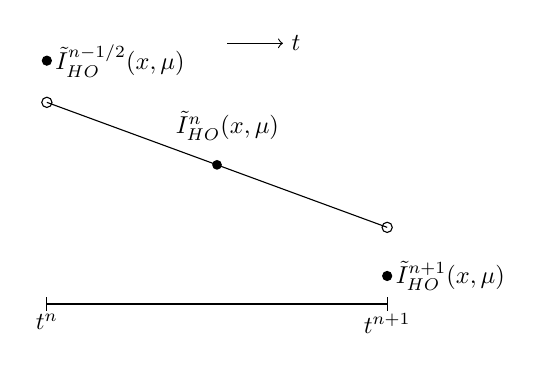
\begin{tikzpicture}[scale=0.882, every node/.style={transform shape}]
            \draw (1.0,4.0) node[fill,circle,inner sep=0pt,minimum
            size=4.2pt] {};
            \node[anchor=west] at (1.0,4.0) {${\tilde{I}_{HO}^{n-1/2}(x,\mu)}$};
            \draw (3.45,2.5) node[fill,circle,inner sep=0pt,minimum size=4.0pt] {};
            \draw [->] (3.6,4.25) -- (4.4,4.25) node[anchor=west] {$t$};
            \draw (1.0,0.4) -- (1.0,0.6) node[below, pos=0.4] {$t^{n}$};
            \draw (5.90,0.4) -- (5.90,0.6) node[below, pos=0.4] {$t^{n+1}$};
            \node at (3.6,3.06) {$\tilde{I}_{HO}^{n}(x,\mu)$};
            \filldraw[color=black, fill=white] (5.9,1.6) circle (2.1pt);
            \draw [thick] (1.0,0.5) -- (5.9,0.5) node[anchor=north west] {};
            \filldraw[color=black, fill=white] (1,3.40) circle (2.1pt);
            \draw (1.0,3.40) -- (5.90,1.6);
            \draw (5.9,0.9) node[black,fill,circle,inner sep=0pt,minimum size=4.2pt] {};
            \node[anchor=west] at (5.9,0.9) {${\tilde{I}_{HO}^{n+1}(x,\mu)}$};
        \end{tikzpicture}
        \caption{\label{fig:ld}LDD trial space}
    \end{subfigure}
    \caption{Illustration of the time variable for $\tilde I_{HO}(x,\mu,t)$ with two unique trial spaces.}
\end{figure}

The second trial space is the LDD trial space in time, as illustrated in
Fig.~\ref{fig:ld}, with an LDFE representation in $x$ and $\mu$.  For a particular space-angle-time element, this trial space is defined as
\begin{multline}
\tilde I(x,\mu,t) = \left \{ \begin{array}{cl}
    \tilde I_{ij}^{n-1/2}(x,\mu) &  \quad t=t^{n-1/2}, \\
    \tilde I_{ij}^n(x,\mu) + \frac{2}{\Delta t}I_{t,ij}^n\left(t-t^{n}\right), &
          t\in (t^{n-1/2},t^{n+1/2}), \\
          \tilde I_{ij}^{n+1/2}(x,\mu) & \quad t=t^{n+1/2}
\end{array}
    \right.
\end{multline}
where  $\tilde I_{ij}^n(x,\mu)$ is the time-averaged LDFE projection in $x$ and $\mu$ over
$\mathcal{D}_{ijn}$ and $I^n_{t,ij}$ is the finite-element slope of $I(x,\mu,t)$ averaged over $\mathcal{D}_{ijn}$,
i.e.,
\begin{equation}\label{eq:tslope}
    I_{ij}^n = \frac{6}{\Delta t} \iiint\limits_{\mathcal{D}_{ijn}} \left( \frac{t - t^{n}}{\Delta
    t} \right) I(x,\mu,t) \,\d x \d \mu \d t.
\end{equation}
Thus, there is a unique time slope for each element.

We will also test problems for an LD trial space in time.  The only difference
from the LDD trial space is that there is no discontinuity at $t^{n+1/2}$. 
To compute consistency terms and advance to the
next time step, the LD approximation of $\tilde
I(x,\mu,t)$ is simply evaluated at $t^{n+1/2}$, extrapolating to the end of the time step. This
introduces an additional approximation error for $I^{n+1/2}(x,\mu)$, and leads to a HO solution that does not as closely
satisfy the exact moment equations (e.g., Eq.~\eqref{eq:t_moml_ex}), as accurately as the LDD trial space.  This
inconsistency can lead to instabilities in the LO equations for rapidly varying solutions. 



\subsection{The Algorithm}

The transport equation to be solved by ECMC is given by Eq.~\eqref{ho_cont}, but with a
fixed LDFE Planckian emission source that is estimated by the previous LO solve.  We write the equation in
operator notation as
\begin{equation}\label{te_oper}
    \B L I(x,\mu,t)  = q_{LO}(x)
\end{equation}
where $q_{LO} = \sigma_a a c \left(T^{n+1/2}\right)^{4}_{LO}/2$ denotes the latest estimate of the
emission source, and remains constant for the entire HO solve. 
The \emph{continuous} linear transport operator $\B L$ is
\begin{equation}\label{L_oper}
   \B L I(x,\mu,t) \equiv \left[ \frac{1}{c}\pderiv{}{t} + \mu \pderiv{}{x} + \sigma_a
    \right] I(x,\mu,t).
\end{equation}
The $m$-th approximate solution to Eq.~\eqref{te_oper} is $\tilde{I}^{(m)}(x,\mu,t)$, where
$m$ identifies the MC batch. The $m$-th residual is 
\begin{equation}\label{eq:res}
r^{(m)} = q - \B L\tilde{I}^{(m)}.
\end{equation}
 Addition
of the residual equation to Eq.~\eqref{te_oper} gives the error equation
\begin{equation}\label{eq:err}
\B L (I - \tilde{I}^{(m)}) = \B L {\epsilon}^{(m)} = r^{(m)},
\end{equation}
where $I(x,\mu,t)$ is the exact solution to Eq.~\eqref{te_oper} (which contains approximation error from the representation of
$\tilde I^{n-1/2}(x,\mu)$ and $q_{LO}$), and ${\epsilon}^{(m)}$ is the error in
$\tilde{I}^{(m)}$. 

The inverse of $\B L$ in Eq.~\eqref{eq:err} is estimated via MC simulation without discretization
error.  This is a standard MC simulation, where particle histories are tracked in space, angle, and
time, e.g., in IMC~\cite{fnc,wollaber_review,dissertation}.
Particle histories are sampled from the source $r^{(m)}(x,\mu,t)$, as explained below.
 Tallies of the error particles estimate 
moments of $\epsilon^{(m)}$, which are added to the moments used to construct the finite-element
representation 
$\tilde{I}^{(m)}$. In operator notation, we denote this as $\tilde{\epsilon}^{(m)} = \B L^{-1}
r^{(m)}$.    The LDFE projections of the
error $\overline{\epsilon}$ and $\epsilon^{n+1/2}$ are computed using generalizations of volumetric
path-length and particle density estimators. The estimators are weighted by appropriate basis
functions over each element.  For the algorithm with the SDD trial space, particles are allowed to stream without
interaction, and the tallies are adjusted accordingly~\cite{bolding_nse}.  
The details of the tallies specific to this work are given in Sec.~\ref{app:tallies}

  The ECMC algorithm is
\begin{enumerate}
    \item Initialize $\tilde I^{(0)}(x,\mu,t)$ with $\tilde I^{n-1/2}(x,\mu)$.
\item Compute $r^{(m)}$.
\item Estimate $\tilde{\epsilon}^{(m)} = \B L^{-1} r^{(m)}$ with $N$ Monte Carlo histories.
\item Compute $\tilde I^{(m+1)} = \tilde I^{(m)}
+ \tilde\epsilon^{(m)}$
\item Optionally repeat 2 -- 4 for desired number of batches.
\end{enumerate}

The use of $\tilde I^{n-1/2}(x,\mu)$ as the initial guess greatly increases statistical efficiency
in regions of the problem where the solution is slowly varying.  For the LDD and LD trial spaces, we also
initialize the time slopes with the corresponding values from the previous time step. If the error is sufficiently
estimated each batch, both statistically and with the projected trial-space representation, then the overall 
error in the solution can converge at an exponential rate.  However, eventually the estimated projection of
the error is not sufficiently accurate  and adaptive refinement would be necessary to continue convergence.  
It is not clear what the best approach to adapt the solution in time is, or if it is practical.   
Thus, we are
primarily only gaining the residual benefit for the algorithm in this work, although in some cases multiple
batches can improve overall efficiency over a single batch.  

A drawback of this HO algorithm is that
a truncation error occurs by keeping only the LDFE projection of the intensity between
time steps, which is not present in IMC.  Adaptive mesh refinement is likely necessary to
efficiently capture rapidly-varying solutions, but this was not done here for simplicity.  
Adaptive refinement in space and angle could be included in the iterative algorithm in future work, which has been
demonstrated for the time-discrete algorithm previously in~\cite{bolding_nse}.  This would also help
minimize memory requirements.

\subsection{Sampling from the Residual}

\subsubsection{The SDD Trial Space}

Computing and sampling from the residual defined by Eq.~\eqref{eq:res} is similar to the sampling algorithms
for a steady-state transport equation~\cite{jake,jake_thesis,bolding_nse}. 
The discontinuities in Eq.~\eqref{eq:time_space} introduce $\delta$-function sources at $t^{n-1/2}$ and $t^{n+1/2}$
because of the time derivative.  Additionally, the residual has a spatial $\delta$-function source
on the upwind face of each element (resulting from the spatial
derivative in the streaming term), and a 2D linear, interior volumetric source.
The contribution from the $\delta$-function source at $t^{n+1/2}$ can be analytically
determined because all particles born immediately reach census~\cite{dissertation}.  Thus, it is never sampled, and the
contribution is added in at the end of the simulation.  

Because the residual can be negative, particles can be sampled with both negative and positive weights.  The
particles are sampled from $|r(x,\mu,t)|$ using rejection sampling over each element. The weights are
modified to be negative if $r(x,\mu,t)<0$ for the sampled phase-space position.
Starting particle weights are normalized to have a magnitude of unity.  The 
final tallies are then multiplied by $\|r(x,\mu,t)\|_1$, the L$_1$ norm of the residual over the entire
sampling domain.  Because of the choice of the SDD trial space, the most complex L$_1$ integral is
the two-dimensional integral of a linear function.  Thus, the L$_1$ norm over all sampling space can be analytically
evaluated, as in previous work~\cite{jake}. To reduce variance in optically
thick regions, systematic sampling~\cite{shultis_mc} is performed, with particles placed proportional to the magnitude
of the residual over each element, as in~\cite{bolding_nse}.  Then the choice of a volumetric or either
$\delta$-function source within the element is discretely sampled, and the corresponding probability
distribution function (PDF) sampled with rejection.  
%Although excluded from the results in this work, a minimum
%number could be placed on each sampled cell to ensure sufficient sampling of the phase space.
%
\subsubsection{The LD and LDD Trial Spaces}

Sec.~\ref{app:res} provides a definition of the residual for the LDD trial space.
The only difference between the residual for the LDD and LD trial spaces is the discontinuity source
at $t^{n+1/2}$, which is analytically treated as for the SDD trial space.
Unlike the SDD trial space, we can not evaluate the L$_1$ norm of the residual analytically.
Additionally, the higher-dimensional residual terms will generally be less efficient to sample with rejection, at
least for certain elements.  Alternatively, we can use importance sampling~\cite{shultis_mc} with
unnormalized particle weights to estimate the magnitude of the
residual.
Previous work on higher-dimensional residual MC has  applied a similar approach for a continuous
global polynomial expansion trial space~\cite{favorite_ecmc}.  Because the solution is continuous, except for at the
boundary, a uniform sampling can be performed over the entire domain and boundary, with weights that
correct for the bias and estimate the magnitude of the residual.  Because our finite element space
contains spatial and temporal discontinuities for each element, particles should be distributed more
closely to the true residual.  Additionally, because $\tilde I^{n-1}(x,\mu,t)$ is typically a good
approximation to $I(x,\mu,t^{n})$, uniform sampling of the domain is very inefficient for thermal
radiative transfer problems.

To apply the importance sampling algorithm, we sample from a simpler distribution function that can
correctly be normalized to a PDF.  The chosen PDF represents a decent
approximation to the residual.  For each element, the new PDF to be sampled from is a piece-wise constant function, spanning the
same domain as the true residual, i.e., including two $\delta$ functions, with their
corresponding subsection of the domain, and the full domain $\mathcal{D}_{ijn}$ (for the interior
source).  The probability of sampling a particular constant source is proportional
to an approximation of the L$_1$ norm of the residual over that element.  The L$_1$ norm is
approximated with product 2-point Gaussian quadratures over each piece of the residual domain.
Thus, the PDF for an element becomes
\begin{equation}
\begin{array}{cl}
    p_{ij}^n(x,\mu,t) &= \ds \frac{\ds \|r\|_{1,i\pm1/2j}^n}{\ds \|r\|_1\Delta t \Delta \mu}\delta^{\mp}\left(x - (x_{i}
    \pm \frac{\ds h_i}{\ds 2})\right) \\ &+ \quad  \frac{\ds \|r\|_{1,ij}^{n-1/2}}{\ds \|r\|_1\Delta x \Delta
    \mu}\delta^{+}\left(t - t^{n-1/2}\right) \\ &+ \quad  \frac{\ds \|r\|_{1,ij}^n}{\ds \|r\|_1\Delta t \Delta \mu \Delta
    x},\quad  (x,\mu,t) \in \mathcal{D}_{ijn} ,
    \end{array}
\end{equation}
where $\|r\|_1$ is the L$_1$ norm of $r(x,\mu,t)$ over the entire domain,
$\|r\|_{1,i\pm 1/2j}^n$ is the norm of the spatial $\delta$-function portion of the element residual
(where the $\pm$ sign corresponds to the direction of $\mu$ for the element),
$\|r\|_{1,ij}^{n-1/2}$ is
the norm of the temporal $\delta$-function portion of the residual, and$\|r\|_{1,ij}^n$ is the norm
of the residual over the interior of the element domain;
all of these norms are approximated with quadrature. Particles are trivially sampled from $p(x,\mu,t)$ and particle weights are initialized as
\begin{equation}
    w(x,\mu,t) = \frac{r(x,\mu,t)}{p(x,\mu,t)}.
\end{equation}
Although the quadrature
approximation may be poor in regions of the domain where zero-crossings of the residual occur, the
overall sampling algorithm is unbiased.  We expect that for reasonably fine meshes the locations of particle
origins are sufficiently proportional to the magnitude of the residual.  
%It is noted that low-variance
%samples of the source do not guarantee low variance in the tallies overall, particularly in thin
%regions.  
High relative variance in weights of particles can also lead to large variances in the
tallies~\cite{shultis_mc}.  However, the slope tallies and extrapolated solution should help produce less noise than the census
tallies of the SDD trial space overall.
As before, we stratify based on $p(x,\mu,t)$ to place particles proportional
to the total probability of sampling from each element and adjust the weights to account for
sampling of integer number of histories.


%%%%%%%%%%%%%%%%%%%%%%%%%%%%%%%%%%%%%%%%%%%%%%%%%%%%%%%%%%%%%%%%%%%%%%%%%%%%%%%%
\section{Results and Analysis}

We have simulated three 1D, grey test problems to demonstrate the efficacy of our HOLO
algorithm: a near-void problem, an optically thin problem, and a standard Marshak wave problem.
We will compare sample statistics and accuracy of solutions to an IMC code with
source tilting~\cite{jayenne} and the HOLO algorithm with BE time-discretized
equations~\cite{bolding_nse}. Throughout this section, results that use the
BE time discretization are indicated with HOLO-BE, and results with the MC-based time
closure are indicated with HOLO-LD, HOLO-LDD, or HOLO-SDD, corresponding to the chosen temporal trial space. 
All plotted results depict the LO solution from the HOLO algorithm.  Some figures depict an
effective radiation temperature defined as $T_{r}(x) = \left(\phi(x)/ac\right)^{1/4}$

To provide a quantitative measure of statistical efficiency, a spatially integrated 
measure of variance in cell-averaged radiation energy
densities $E_{r,i}^{n+1/2}$ was computed, based on the solution at the simulation end time.
To form sample estimates of the variance in the cell-averaged values, twenty independent simulations for each
particular result and method were performed.% using unique random number generator seeds.
The sample variance for a particular cell-averaged $E_{r,i}^{n+1/2}$ is 
\begin{equation} 
    S_i^2 =  \frac{20}{20-1} \sum_{l=1}^{20} \left(\overline{E^{n+1/2}_{i}} -
    E_{r,i}^{n+1/2,(l)}\right)^2,
\end{equation}
where $E_{i}^{n+1/2,(l)}$ is the cell-averaged scalar intensity for cell $i$ from the $l$-th of 20 independent simulations, and
$\overline{E^{n+1/2}_{i}}$ is the corresponding sample mean, from the 20 simulations. To
provide a normalized, spatially-integrated result, we form a norm over cells as 
\begin{equation}
    \ss = \left({\frac{\ds \sum\limits_{i=1}^{N_c}
S_i^2}{\ds \sum\limits_{i=1}^{N_c}\left(\overline{E_{r,i}^{n+1/2}}\right)^2}}\right)^{1/2},
\end{equation}
where $N_c$ is the number of spatial elements. We use this statistic to form a figure of merit (FOM) to demonstrate how statistical accuracy
scales with the number of histories performed.  Our FOM is defined as
\begin{equation}\label{eq:fom}
    \FOM = \frac{1}{N_{\text{tot}}\ss^2}
\end{equation}
where $N_{\text{tot}}$ is the total number of histories performed during a particular simulation.
A larger value of the FOM indicates that the method produced less variance in the
solution, per history performed, for a given problem.  This form of the FOM
is typically chosen because the variance is expected to reduce inversely proportional
to $N_{\text{tot}}$, so for standard MC simulations the FOM becomes, on average, independent of
$N_{tot}$~\cite{shultis_mc}.  The FOM is not necessarily expected to be independent
of $N_{\text{tot}}$ for the HOLO method because of correlations in the ECMC solver.
It is difficult to compare computational times with the IMC method because they are implemented in
different code infrastructures.  Additionally, the HOLO algorithm is converging nonlinearities,
whereas the IMC method is only taking a single linearized step, for each time step.  Thus, we only
focus on the reduction in overall variance, per particle history, as a measure of efficiency.

We have also compared against IMC for accuracy for the optically thin problem. An
integral error in cell-averaged energy densities for the
$l$-th simulation, with $N_c^{(l)}$ spatial cells, is computed as
\begin{equation}\label{eq:avg_err}
    \|e\|^{{(l)}}_{a,rel} = \left({\frac{\ds \sum\limits_{i=1}^{N^{(l)}_c}
    \left(E_{r,i}^{n+1/2,{(l)}} - E_{r,i}^{n+1/2,ref}
\right)^2}{\ds \sum\limits_{i=1}^{N^{(l)}_c}\left(E_{r,i}^{n+1/2,ref}\right)^2}}\right)^{1/2},
\end{equation}
where $E_{r,i}^{n+1/2,ref}$ is computed by spatially averaging the reference IMC solution over
the $i$-th coarse spatial cell, with the assumption of uniform mesh spacing.


\subsection{Near-Void Problem}


\begin{figure*}[bth!]
\centering
\begin{subfigure}{0.48\textwidth}
  \centering
  \vspace{-0.051in}
    \captionsetup{justification=centering,margin=1.5cm}
    \includegraphics[width=0.96\textwidth]{void_imc_compare.pdf}
    \caption{\label{fig:void_imc_compare} Radiation energy densities $E_{r,i}$  with
    $\Delta t=0.001$ sh.}
\end{subfigure}
\begin{subfigure}{0.48\textwidth}
  \centering
    \captionsetup{justification=centering,margin=1.0cm}
    \includegraphics[width=\textwidth]{void_temp_batch_compare.pdf}
    \caption{\hspace{0.1in}\label{fig:void_temp_compare} Radiation temperatures $T_{r,i}$ for
    different time step sizes and numbers of batches.}
\end{subfigure}
\begin{subfigure}{0.52\textwidth}
  \centering
    \includegraphics[width=\textwidth]{void_ang_compare.pdf}
    \caption{\label{fig:bumps} Census radiation energy densities $E_{r,i}^{n+1/2}$ for
    the HOLO-LDD method with different numbers of $\mu$ cells and $\Delta t=0.001$ sh.
}
\end{subfigure}
\caption{Comparisons between IMC and the HOLO method with different time discretizations and
settings.}
\end{figure*}  

For the first problem, the material properties
are uniform throughout a 2.0-cm wide domain with $\rho c_v = 0.01374$ GJ cm$^{-3}$ keV$^{-1}$, $\sigma_a=10^{-6}$ cm$^{-1}$.
The near-void cross section essentially uncouples the material and radiation.  
The material and radiation are initially in equilibrium at a temperature of $0.01$ keV.
An isotropic incident intensity with $T_r = 0.150$ keV is applied
at $x=0$ for $t>0$; the incident intensity on the right boundary is $0.01$ keV.  The simulation end
time is $t=0.003$ sh.  

A comparison of the cell-averaged radiation energy densities $E_r$ for IMC and the HOLO
method with different time closures is depicted in Fig.~\ref{fig:void_imc_compare};
values for the time-averaged and $t^{n+1/2}$ energy densities, from the final time
step, are given.  The end of time step value for the HOLO method with a BE discretization is also depicted.
Three relatively large time steps are taken with $\Delta t = 0.001$ sh.
For the HOLO results, three ECMC batches were performed with
a total of $3\times10^6$ histories per time step, and the IMC results were generated with
$3\times10^6$ histories per time step.
The spatial meshes had 100 spatial cells and all HOLO results used 30 $\mu$ cells.  
The MC treatment of the time
variable and the closure of the LO equations allow the LO results to correctly reconstruct
the wave-front location of IMC, whereas the BE discretization artificially propagates
energy. This problem is nearly linear due to the small cross sections, so the HO time closures are
stable and correctly reproduce the time-averaged and $t^{n+1/2}$ HO moments, even for the large time steps of this problem.
This problem represents a limiting case where IMC is more efficient and accurate.  Because the IMC particles are only 
streaming, the space of the initial source is all that must be sampled, whereas the ECMC algorithm must resample
the distribution and residual space each time step.

A comparison of HOLO-SDD solutions with variable numbers of batches and time step sizes, but the
same total $9\times10^6$ histories for each simulation, is given in Fig.~\ref{fig:void_temp_compare}.  Results are 
depicted as radiation temperatures.  By plotting
proportional to the fourth-root of the radiation energy density, the noise at low
magnitudes past the wave-front are more apparent for the 3 batches and $\Delta t = 0.001$ sh
case.  This noise is minimal relative to the scale of $E_r$, but it demonstrates a
deficiency of the residual method.  The representation over
the time step leads to particles sampled near the wave-front with a time near
$t^{n}$ that travel into the equilibrium region.  This is not a
bias, but rather an under-sampling of the phase space; if sufficient histories were performed there
would be negative particles that canceled out this error. The ECMC iterations can also lead to small negative
averages for the HO solution in the equilibrium region.   In such cells, the
average was set to the floor value and slopes to zero. For the case of a single batch, 
there is less noise past the wavefront because the
choice of $\tilde I^{n-1/2}(x,\mu)$ as an initial guess for $\tilde I^{n}(x,\mu,t)$ prevents most particles from
traveling past what the physical transport should allow.

The noise in the equilibrium region is significantly reduced by taking a smaller time step, although
the mesh-imprinting error is increased.  The mesh-imprinting error is a discretization effect
resulting from only storing a projection between time steps.  
Fig.~\ref{fig:bumps} illustrates the convergence of this
effect as a function of the number of angular elements used, for the HOLO-LDD method.
At coarser mesh sizes, the imprinting of the mesh is visible in the location of
the wavefront, although the location of the wavefront is accurate.  
Smaller time step sizes can increase the mesh imprinting because a more difficult to resolve solution is being projected
more often.  The error is reduced as the mesh is refined.  Generally, the imprinting is reduced as $\sigma_a$ is increased and
absorption-emission events smooth the angular intensity across each time step.


\subsection{Optically-Thin Problem}

We modify the near-void problem by increasing the absorption cross section to 0.2
\invcm; all other problem parameters are the same.  Radiation temperatures at the end of
the last time step are compared in Fig.~\ref{fig:thin_temp_compare} for the IMC and various HOLO
methods. The HOLO results were generated with 30
$\mu$ cells, and all spatial meshes used 100 cells.  All results used $3\times10^6$
histories per time step.   There is good agreement between
the HOLO-LDD and HOLO-SDD results with IMC, except some dispersion past the wavefront.
This dispersion is caused by the spatial discretization inconsistency between the LDFE HO projection and the
lumped LDFE LO equations; this dispersion is not present in the HO solution. 
As in the previous problem, the HOLO-BE results are very
inaccurate at capturing the wavefront location. 
IMC demonstrates substantial statistical noise in the equilibrium region.
The HOLO-LD method is unstable for this problem.  This is caused by inconsistency between the HO and
LO space-angle-time moment equations.  In particular, the approximation of $I^{n+1/2}(x,\mu)$ via extrapolation based on the
interior slope leads to an unstable closure relation.   At lower history counts, the other HOLO
methods can become unstable as well.
\begin{figure}[h!]
  \centering
    \includegraphics[width=0.49\textwidth]{thin_temp_compare.pdf}
    \caption{\label{fig:thin_temp_compare} Comparison of radiation temperatures of IMC and
    the HOLO method for different time step sizes and numbers of batches, for optically
thin problem. }
\end{figure}

The value of $\|e\|_{a,rel}$ was computed by averaging the computed value of Eq.~\eqref{eq:avg_err}
from 20 simulations.  The IMC method and various HOLO methods are compared against a reference IMC
solution. Because the material is loosely coupled in this problem, we expect IMC to be accurate with
sufficient particle
histories.  The
reference solution is the average of 20 IMC simulations of $20\times10^6$
histories, each with $\Delta t =10^{-4}$ sh.  The estimated value of $\ss$ for the
reference solution is 0.025\%.  Sample statistics are also compared via the $\FOM$
from Eq.~\eqref{eq:fom}.

Table.~\ref{tab:thin_short} compares values of the FOM and $\|e\|_{a,rel}$ for $\Delta t=10^{-4}$
sh.  The results in the table are for 200 spatial cells, computed against a reference solution with 100 spatial cells.
The HOLO results were generated with a single batch per time step, although similar accuracy was found for the case
of two batches (with the same number of histories per time step).   
 All FOM values are normalized to the IMC result with 
200 $x$ cells and 30,000 histories. 

The HOLO method, with sufficient histories to prevent instabilities, is more accurate and
substantially more efficient.     For reference, statistics were measured for the HOLO-BE method with two batches of 150,000
histories per time step, producing $\|e\|_{a,rel}=10.5\%$ and $\FOM=3100$, demonstrating
substantial inaccuracy but improved efficiency.
 For 100 $x$ cells, the projection error limits accuracy and the
IMC method becomes more accurate.
\begin{table}[H]
\centering
\caption{\label{tab:thin_short} {Comparison of $\|e\|_{a,rel}$ and $\FOM$ values for the end of time
    step radiation energy densities, of the last time step, for the optically
    thin problem, 200 $x$ cells, and $\Delta t = 1\times 10^{-4}$ sh.  The reference IMC result has 100 $x$ cells.
    Simulation end time is ${t=0.003}$ sh. Fractional error in all results  below 0.01}}
\begin{tabular}{|c|ccc|}\cline{1-4}
    \multicolumn{4}{|c|}{$\mathbf{\|e\|_{a,rel}}$} \\ \hline
hists./step   & IMC     & HOLO-SDD  &  HOLO-LDD \\ \hline
   30,000     & 2.93\%   & 14.00\%   & 14.50\%      \\
  300,000     & 0.99\%   & 0.37\%    &  0.46\%      \\ 
  1,000,000   & 0.49\%   & 0.18\%    &  0.19\%       \\ \hline
    \multicolumn{4}{|c|}{\textbf{\FOM}} \\ \hline
hists./step   & IMC    & HOLO-SDD  &  HOLO-LDD \\ \hline
   30,000     & 1      &  0.11  & 0.10 \\
  300,000     & 0.90   &  14.24 & 8.61 \\
  1,000,000   & 1.01   &  81.71 & 71.36 \\\hline
  \end{tabular}
  \end{table}

\subsection{Marshak Wave Problem}

It is important to demonstrate that the time closures are stable in a mix of optically-thick and
optically-thin regions and that the ECMC method is still efficient for such
problems.  This problem has the same material properties as the optically thin problem except for a
temperature-dependent cross-section with
$\sigma_a(T) = 0.001 T^{-3}$ and the initial temperature is $2.5\times10^{-5}$ keV.  The time step size is linearly increased from $0.001$ sh to a
maximum step of 0.01 sh over the first 10 time steps. 
It was found for this problem that it was
necessary to use more than one batch for the HOLO-SDD and HOLO-LDD methods and large numbers of
histories to stably converge, as it is difficult
for particles to reach the end of the time step.  A second batch results in a better initial approximation
for $I^{n+1/2}$, resulting from the extrapolated interior solution of the first batch.
Thus, all HOLO results in this section use two batches.
\begin{figure}[H]
    \centering
    \includegraphics[width=0.49\textwidth]{marshak_time_cont_compare.pdf}
    \caption{\label{fig:marshak_tc} Comparison of HOLO-TC, HOLO-BE, and IMC methods for
the Marshak Wave problem, with $10^6$ histories per time step.}
\end{figure}

Figure~\ref{fig:marshak_tc} compares the accuracy of IMC and the various HOLO methods, showing
agreement between the solutions. There were $10^6$ histories per time step for all
simulations. This slowly varying problem can be accurately modeled with the BE time discretization, but
the MC time closures are stable.  Because the problem is slowly-varying, the HOLO-LD method was found to stably
converge, without the need for the second discontinuity.  The HOLO-LD method is sufficiently
consistent because for this problem $\tilde I^n(x,\mu) \simeq I^{n+1/2}(x,\mu)$.

Table~\ref{tab:marshak_cont} compares sample statistics for IMC,
the HOLO-LD, HOLO-SDD, and the HOLO-BE
method. The FOM values are relative to IMC with 300,000 histories per time
step.  The HOLO-BE method is significantly more efficient for comparable accuracy in this
problem. The HOLO-LD method is much more efficient than the HOLO-SDD method because the LD trial space does not require error estimates at $t^{n+1}$.
The doubly-discontinuous trial spaces were found to be exceptionally noisy for this problem, 
requiring $10^6$ histories per time step to remove visible noise, although they were still more
efficient than standard IMC, as demonstrated by the FOM.  At $300,000$ histories per time step the
SDD trial space converges, but has large noise and inaccuracies due to oscillations introduced
through noise in the time closure.
\begin{table}[H]
\centering
\caption{\label{tab:marshak_cont} {Comparison of FOM for the Marshak
    wave problem.  Simulation end time is $\mathbf{t=3.0}$ sh.}}
\begin{tabular}{|c|cccc|}\cline{2-5}
    \multicolumn{1}{c|}{}        &
    \multicolumn{4}{|c|}{\FOM} \\ \hline
hists./step    &  IMC   & HOLO-SDD  & HOLO-LD  & HOLO-BE    \\ \hline
   50,000      &  0.92  &   --         &  96.2      & 1708             \\
  300,000      &  1.00  &   0.43       &  200     & 2050         \\  
  1,000,000    &  0.94  &  15.95       &  201     & 1806          \\ \hline
\end{tabular}
\end{table}

%%%%%%%%%%%%%%%%%%%%%%%%%%%%%%%%%%%%%%%%%%%%%%%%%%%%%%%%%%%%%%%%%%%%%%%%%%%%%%%%
\section{Conclusions}

We have extended a HOLO method to include a residual MC treatment of the time variable, producing
accurate solutions to simplified TRT problems..
Results demonstrate that the inversion of the transport operator in the residual MC algorithm allows
for an accurate projection of the solution across time steps, increasing accuracy in optically thin
regions compared to a BE discretization.  For most cases tested, a single batch simplifies the
sampling space and leads to less variance overall than iterating on the residual.  For optically
thin problems, moments of the LO
solution were found to agree with IMC when used with the LDD and SDD HO trial
spaces; the HOLO method was more accurate and efficient
than IMC, although sufficient mesh resolution is needed to limit projection error between time
steps.  For the Marshak wave problem, our ECMC algorithm is more statistically
efficient than IMC, although the solution is not guaranteed to converge at lower particle history counts.
 We have demonstrated a new approach to closing the LO equations in time that produces
accurate solutions with a HO solver that is sufficiently consistent.  For the Marshak wave problem,
the LD trial space in time is significantly more efficient than the doubly-discontinuous trial
spaces, but inconsistencies lead to instabilities for thinner problems and finer meshes. Overall,
each of the trial spaces has desirable and negative properties for a certain set of problems.

Future investigation of time-integration for this algorithm should include investigation of convergence in outer iterations when
incorporating a time-averaged projection of the physical scattering source into the LO solver.
Also, adaptive refinement in space and angle should be used to more accurately capture transient
solutions.  Investigation of the practicality and approach for adapting in time is necessary for
obtaining a true ECMC algorithm with time-dependent transport equations.
Second-order time-integration methods for the temperature could be incorporated.  Although they will
require solving a more difficult set of LO equations, the cost of the HO solver with the LDD trial
space should be unaffected.
Long-term, an ideal algorithm
would require no projection of the HO solution between time steps, as in IMC, which will likely require an operator split
on the radiation time derivative and a method to map the projected error back on to
the census particles.  Finally, the new sampling strategy for the LDD and LD trial spaces should be
applied to higher-dimensional problems.  Because of the difficulties with consistency and
exceptionally difficult to resolve gradients in TRT problems, steady-state neutronics problems
should be investigated first.

%%%%%%%%%%%%%%%%%%%%%%%%%%%%%%%%%%%%%%%%%%%%%%%%%%%%%%%%%%%%%%%%%%%%%%%%%%%%%%%%
\appendix
\section{Appendix}

\subsection{The Residual for the LDD Trial Space}
\label{app:res}

The LDFE representation for the element with center $(x_i,\mu_j, t^n)$, spanning the interior of the domain
$\mathcal{D}_{ijn}$, is 
\begin{equation}\label{ld_full}
    \tilde I(x,\mu,t) = I_{a,ij}^{n} + \frac{2}{h_{i}}I_{x,ij}^{n}\left(x-x_i\right) +
    \frac{2}{\Delta \mu}I_{\mu,ij}^n\left(\mu-\mu_j\right) +
    \frac{2}{\Delta t}I_{t,ij}^{n}\left(t-t^{n}\right)
\end{equation}
where $\Delta \mu = \mu_{j+1/2} - \mu_{j-1/2}$ and $I_{a,ij}^n$, $I_{x,ij}^n$, $I_{\mu,ij}^n$, and 
$I_{t,ij}^n$ are the average, $x$ slope, $\mu$ slope, and $t$ slope moments,
respectively~\cite{dissertation}.   We substitute
Eq.~\eqref{ld_full} into Eq.~\eqref{eq:res} and analytically apply the continuous transport operator to determine the
residual.  For each cell, the residual is the sum of four components.  The first is the interior volumetric source:
\begin{equation}
    r_{ij}^{n}(x,\mu,t) = r_{a,ij}^n + \frac{2}{h_i}r_{x,ij}^n\left(x-x_i\right) + 
    \frac{2}{\Delta \mu}r_{\mu,ij}^n\left(\mu-\mu_j\right) +
    \frac{2}{\Delta t}r_{t,ij}^{n}\left(t-t^{n}\right)
\end{equation}
where
\begin{align}
    r_{a,ij}^n &= q_{a,i} - \sigma_{a,i}I^n_{a,ij} - \frac{2}{c \Delta t} I_{t,ij}^n - \mu_{j}\frac{2}{\Delta
    \mu}I_{x,ij}^n, \\ 
    r_{x,ij}^n &= q_{x,i} - \sigma_{a,i}I^n_{x,ij}, \\ 
    r_{\mu,ij}^n &= -\sigma_{a,i}I^{n}_{\mu,ij} - \frac{\Delta \mu}{h_{i}}I^{n}_{x,ij}, \\
    r_{t,ij}^n &= -\sigma_{a,i}I^{n}_{t,ij}
\end{align}
where $q_{a,i}$ and $q_{x,i}$ are the zeroth and first moments of the LO LDFE emission source over the
$i$-th spatial element ($q_{LO}(x)$ does not have a first moment in $\mu$ or $t$).  The spatial derivative produces a
$\delta$-function source due to the discontinuities in the trial space. Upwinding is used to define the
intensity on the inflowing face.  The face source component, for $\mu>0$, becomes
\begin{multline}
    r_{i-1/2j}^{n} = \delta^+(x-x_{i-1/2}) \mu \left[ r_{a,ij}^{n,f}  \right.
 \\   \left. + \frac{2}{\Delta \mu} r_{\mu,ij}^{n,f} \left(\mu - \mu_j\right) +
    \frac{2}{\Delta t}r_{t,ij}^{n,f}\left(t - t^{n}\right)\right] 
\end{multline}
where
\begin{align}
    r_{a,ij}^{n,f} &= \left(I_{a,i-1,j}^{n} + I_{x,i-1,j}^n\right) - \left(I_{a,ij}^{n} - I_{x,ij}^n\right)       \\ 
    r_{\mu,ij}^{n,f} &= I_{\mu,i-1,j}^{n} - I_{\mu,ij}^n, \\ 
    r_{t,ij}^{n,f} &= I_{t,i-1,j}^{n} - I_{t,ij}^n.
\end{align}
The face sources for elements with $\mu<0$ are similarly defined.  The time-derivative
jump source at $t^{n-1/2}$ is
\begin{multline}
    r_{ij}^{n-1/2} = \delta^+(t-t^{n-1/2})\frac{1}{c}\left[ r_{a,ij}^{n-1/2}  \right. \\ \left. +  \frac{2}{h_i}
    r_{x,ij}^{n-1/2} \left(x - x_i\right) +
    \frac{2}{\Delta \mu}r_{\mu,ij}^{n-1/2}\left(\mu - \mu_j\right)\right] 
\end{multline}
where
\begin{align}
    r_{a,ij}^{n-1/2} &= I_{a,ij}^{n-1/2} - \left(I_{a,ij}^n - I_{t,ij}^n\right), \\
    r_{x,ij}^{n-1/2} &= I_{x,ij}^{n-1/2} - I_{x,ij}^n, \\ 
    r_{\mu,ij}^{n-1/2} &= I_{\mu,ij}^{n-1/2} - I_{\mu,ij}^n.
\end{align}
Finally, the time-derivative component at $t^{n+1/2}$ is
\begin{multline}
    r_{ij}^{n-1/2} = \delta^-(t-t^{n+1/2})\frac{1}{c}\left[ r_{a,ij}^{n-1/2}  \right. \\ \left. +  \frac{2}{h_i}
    r_{x,ij}^{n-1/2} \left(x - x_i\right) +
    \frac{2}{\Delta \mu}r_{\mu,ij}^{n-1/2}\left(\mu - \mu_j\right)\right] 
\end{multline}
where
\begin{align}
    r_{a,ij}^{n+1/2}   &=   \left(I_{a,ij}^n - I_{t,ij}^n\right) -I_{a,ij}^{n-1/2}, \\
    r_{x,ij}^{n+1/2}   &= I_{x,ij}^{n-1/2}   I_{x,ij}^n, \\ 
    r_{\mu,ij}^{n+1/2} &= I_{\mu,ij}^{n-1/2} I_{\mu,ij}^n.
\end{align}
Particles sampled from this source would immediately reach census and terminate, thus there is no
need to sample it.  The analytic contribution from this source can be added, as detailed
in~\cite{dissertation}, reducing variance.

\subsection{Tallies for the Error}

\label{app:tallies}
Tallies compute weighted moments of the error, averaged over the phase-space volume of each element. 
 For both trial spaces, the time-averaged LDFE projection  $\tilde I^n(x,\mu)$ is computed. 
This requires tallies for the average, $x$, and $\mu$ moments of the
error.  The tally for analog path-length sampling and the $x$ moment of the error is 
\begin{equation}
    {\hat \epsilon}^n_{x,ij} =\frac{1}{N} \frac{6}{\Delta t h_i} \sum_{m=1}^{N_{score}}
    \frac{s_m}{h_{i}\Delta \mu} w_m \left(x^m_c - x_i\right),
\end{equation}
where $x^m_c$ is the center $x$-coordinate of the path length for the $m$-th particle history with
length $s_m$ and constant weight $w_m$, and $N_{score}$ is the number of particles that have traversed the domain
$\mathcal{D}_{ijn}$..  There
are similar definitions for the average and $\mu$ moment.  The tallies are derived by
integrating the contribution of a differential path length, to the moment of interest, over the entire path
length~\cite{dissertation}.  As in previous work, these tallies can be modified to allow for particles that
stream without absorption and have exponentially attenuated weights~\cite{bolding_nse}. 

For the SDD and LDD trial spaces, moments of $\epsilon(x,\mu,t^{n+1/2})$ must be estimated to produce a projection of the intensity at
the end of the time step.
For example, the $x$ moment of the error at the end of time step is
\begin{equation}
    \epsilon^{n+1/2}_{x,ij} = \frac{6}{h_i\Delta \mu \Delta t} \iint\limits_{\mathcal{D}_{ij}} \left(\frac{x
    - x_i}{h_i}\right) \epsilon(x,\mu,t^{n+1/2}) \d x \d \mu
\end{equation}
The estimators for these moments are a generalization of the census
tallies used in IMC~\cite{wollaber_review,fnc}.   The census estimator for the $x$ moment is
\begin{equation}
    \hat\epsilon^{n+1/2}_{x,ij} = \frac{1}{N} \frac{6}{\Delta \mu h_i^2} \sum_{n=1}^{N_{score}}
    c w_m  \left(x_{m} - x_{i}\right),
\end{equation}
where $x_m$ is the coordinate of the $m$-th particle that has reached the end of the time step.
Similar tallies are defined for the other space-angle moments. These tallies can be
exceptionally noisy in optically thick cells because only particles that reach the end of the time step contribute.

For the LDD and LD time spaces, it is necessary to tally the slope of the intensity in $t$ over each
element, i.e., estimate Eq.~\eqref{eq:tslope}.  The estimator, for analog path-length sampling, is
\begin{equation}
    \hat\epsilon^{n}_{t,ij} = \frac{1}{N} \frac{6}{h_i\Delta \mu\Delta t} \sum_{m=1}^{N_{score}} 
    \left(\frac{t_c^m
    - t^n}{\Delta t}\right) w_m s_m
\end{equation}
where $t_c^m$ is the time of the particle at the center of the path length.

%%%%%%%%%%%%%%%%%%%%%%%%%%%%%%%%%%%%%%%%%%%%%%%%%%%%%%%%%%%%%%%%%%%%%%%%%%%%%%%%
\section{Acknowledgments}

This research was supported with funding received from the DOE National
Nuclear Security Administration, under Award Number(s) DE-NA0002376. 

%%%%%%%%%%%%%%%%%%%%%%%%%%%%%%%%%%%%%%%%%%%%%%%%%%%%%%%%%%%%%%%%%%%%%%%%%%%%%%%%
\bibliographystyle{ans} % Don't forget to run BibTeX !
\bibliography{bibliography}

\end{document}

